\documentclass[]{book}
\usepackage{lmodern}
\usepackage{amssymb,amsmath}
\usepackage{ifxetex,ifluatex}
\usepackage{fixltx2e} % provides \textsubscript
\ifnum 0\ifxetex 1\fi\ifluatex 1\fi=0 % if pdftex
  \usepackage[T1]{fontenc}
  \usepackage[utf8]{inputenc}
\else % if luatex or xelatex
  \ifxetex
    \usepackage{mathspec}
  \else
    \usepackage{fontspec}
  \fi
  \defaultfontfeatures{Ligatures=TeX,Scale=MatchLowercase}
\fi
% use upquote if available, for straight quotes in verbatim environments
\IfFileExists{upquote.sty}{\usepackage{upquote}}{}
% use microtype if available
\IfFileExists{microtype.sty}{%
\usepackage{microtype}
\UseMicrotypeSet[protrusion]{basicmath} % disable protrusion for tt fonts
}{}
\usepackage{hyperref}
\hypersetup{unicode=true,
            pdftitle={Medicina Basada en Evidencias},
            pdfauthor={Lujohn Florez, Gener J Avilés-R},
            pdfborder={0 0 0},
            breaklinks=true}
\urlstyle{same}  % don't use monospace font for urls
\usepackage{natbib}
\bibliographystyle{plainnat}
\usepackage{longtable,booktabs}
\usepackage{graphicx,grffile}
\makeatletter
\def\maxwidth{\ifdim\Gin@nat@width>\linewidth\linewidth\else\Gin@nat@width\fi}
\def\maxheight{\ifdim\Gin@nat@height>\textheight\textheight\else\Gin@nat@height\fi}
\makeatother
% Scale images if necessary, so that they will not overflow the page
% margins by default, and it is still possible to overwrite the defaults
% using explicit options in \includegraphics[width, height, ...]{}
\setkeys{Gin}{width=\maxwidth,height=\maxheight,keepaspectratio}
\IfFileExists{parskip.sty}{%
\usepackage{parskip}
}{% else
\setlength{\parindent}{0pt}
\setlength{\parskip}{6pt plus 2pt minus 1pt}
}
\setlength{\emergencystretch}{3em}  % prevent overfull lines
\providecommand{\tightlist}{%
  \setlength{\itemsep}{0pt}\setlength{\parskip}{0pt}}
\setcounter{secnumdepth}{5}
% Redefines (sub)paragraphs to behave more like sections
\ifx\paragraph\undefined\else
\let\oldparagraph\paragraph
\renewcommand{\paragraph}[1]{\oldparagraph{#1}\mbox{}}
\fi
\ifx\subparagraph\undefined\else
\let\oldsubparagraph\subparagraph
\renewcommand{\subparagraph}[1]{\oldsubparagraph{#1}\mbox{}}
\fi

%%% Use protect on footnotes to avoid problems with footnotes in titles
\let\rmarkdownfootnote\footnote%
\def\footnote{\protect\rmarkdownfootnote}

%%% Change title format to be more compact
\usepackage{titling}

% Create subtitle command for use in maketitle
\providecommand{\subtitle}[1]{
  \posttitle{
    \begin{center}\large#1\end{center}
    }
}

\setlength{\droptitle}{-2em}

  \title{Medicina Basada en Evidencias}
    \pretitle{\vspace{\droptitle}\centering\huge}
  \posttitle{\par}
  \subtitle{Una Aproximación Paso a Paso Para el Club de Revistas de Medicina de Estilo de Vida.}
  \author{Lujohn Florez, Gener J Avilés-R}
    \preauthor{\centering\large\emph}
  \postauthor{\par}
      \predate{\centering\large\emph}
  \postdate{\par}
    \date{2019-10-16}

\usepackage{booktabs}
\usepackage{amsthm}
\makeatletter
\def\thm@space@setup{%
  \thm@preskip=8pt plus 2pt minus 4pt
  \thm@postskip=\thm@preskip
}
\makeatother

\begin{document}
\maketitle

{
\setcounter{tocdepth}{1}
\tableofcontents
}
\hypertarget{introduccion}{%
\chapter{Introducción}\label{introduccion}}

Éste manual está diseñado para acompañar las sesiones del Club de Revistas de la Clínica del Estilo de Vida adscrita al Hospital ``La Carlota'', dirigida por el \href{https://www.linkedin.com/in/lujohnflorez/}{Dr Lujhon Flores}.
La aproximación a la teoría de medicina basada en evidencia es compilada y presentada por el \href{https://www.linkedin.com/in/generaviles/}{Dr.~Gener J Avilés-R}.

\hypertarget{intro}{%
\chapter{¿Qué es la medicina basada en evidencias?}\label{intro}}

Originalmente la medicina basada en evidencias (MBE) se definió como el uso conciente, explícito y juicioso de la mejor evidencia disponible para la toma de decisiones sobre la atención individual de pacientes \citep{sackett1996evidence}.
La versión actualizada de éste concepto se definió como:

\begin{quote}
``La integración de la mejor evidencia en \textbf{investigación} con el \textbf{expertiese clínico} y los \textbf{valores del paciente}.'' \citep{straus2018evidence}
\end{quote}

Ésta última definición prioriza una aproximación sistemática a la resolución de problemas clínicos que incluyen al paciente de forma activa, la experiencia del/la clínico y los resultados en investigación. A éste conjunto de características se le ha llamado la \textbf{tríada de la medicina basada en evidencias.}

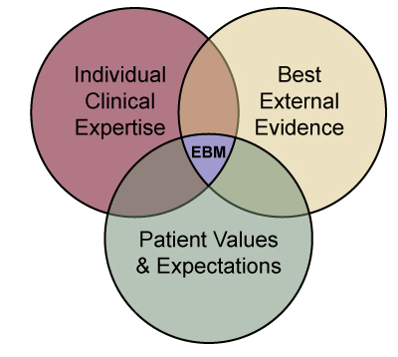
\includegraphics{img/EBM.png}

\hypertarget{que-competencias-de-mbe-necesitan-todos-los-medicos-clinicos}{%
\section{¿Qué competencias de MBE necesitan TODOS los médicos clínicos?}\label{que-competencias-de-mbe-necesitan-todos-los-medicos-clinicos}}

\textbf{Habilidades elementales en MBE.}

A continuación se presenta una lista no exahustiva de las habilidades que tod@ médico clínico debe tener, indistinto de su nivel de especialización o lugar de trabajo \citep{slawson2005teaching}.

\begin{itemize}
\tightlist
\item
  \emph{Information mastery}: la capacidad de encontrar la mejor evidencia para la práctica del día a día.
\item
  Tener información \emph{en tiempo y forma} en el pointo de atención para la toma de decisiones clínicas.

  \begin{itemize}
  \tightlist
  \item
    Basadas en la internet u \emph{offline}.
  \end{itemize}
\item
  Evaluar información generada por expertos, \textbf{incluyendo colegas}, educación médica continua, presentaciones, revisiones y guías.
\item
  Evaluar de forma crítica información de representantes de farmaceúticas y/u otros promotores de terapeúticas alópatas o alternativas.
\end{itemize}

\hypertarget{habilidades-que-solo-un-pequeno-porcentaje-de-medicos-clinicos-necesitan-dominar.}{%
\section{Habilidades que solo un pequeño porcentaje de médicos clínicos necesitan dominar.}\label{habilidades-que-solo-un-pequeno-porcentaje-de-medicos-clinicos-necesitan-dominar.}}

\textbf{Habilidades avanzadas en MBE \citep{slawson2005teaching}.}

\begin{itemize}
\tightlist
\item
  Evaluación crítica e interpretación de investigaciones en:

  \begin{itemize}
  \tightlist
  \item
    Terapias.
  \item
    Procesos diagnósticos.
  \item
    Test diagnósticos.
  \item
    Estudios de pronóstico.
  \end{itemize}
\item
  Evaluación crítica e interpretación de:

  \begin{itemize}
  \tightlist
  \item
    Revisiones sistemáticas (incluyendo meta-análisis),
  \item
    Análisis de decisión,
  \item
    Guías de práctica,
  \item
    Marketing farmaceútico.
  \end{itemize}
\item
  Asignar niveles de evidencia a hallazgos en investigación.
\item
  Enseñanza de competencias elementales en MBE.
\item
  Producir comunicaciones orales y por escrito de hallazgos en investigación.

  \begin{itemize}
  \tightlist
  \item
    Para pacientes.
  \item
    Para colegas médicos.
  \end{itemize}
\end{itemize}

\hypertarget{quienes-deben-aprender-competencias-avanzadas}{%
\subsection{¿Quiénes deben aprender competencias avanzadas?}\label{quienes-deben-aprender-competencias-avanzadas}}

\begin{itemize}
\tightlist
\item
  Médicos que son vistos como líderes de opinión en su campo.
\item
  Clínicos que entrenan a otros médicos.
\item
  Médicos en centros de referencia para su especialidad/línea de práctica clínica.
\item
  Médicos educadores, escritores quienes proveen información para otros consumidores de información clínica.
\item
  \emph{¿Médicos de la \href{http://clinicadelestilodevida.org/}{Clínica del Estilo de Vida}?}
\end{itemize}

\hypertarget{mbe-en-la-practica.}{%
\section{MBE en la práctica.}\label{mbe-en-la-practica.}}

Inicialmente el proceso de la práctica clínica basada en evidencia se realizaba leyendo publicaciones del área de expertiese clínica de interés, el médico dispondría una cantidad de tiempo semanal/diario a leer publicaciones relevantes.

Si ésto fuera la práctica actual sería imposible para el clínico leer todas las publicaciones relevantes de su área de interés y mantener una práctica diaria efectiva.

Otro detalle que surgue al intentar seguir la práctica mencionada es que, la mayoría de los documentos leídos no tendrían relación con los pacientes atendidos en la práctica del día. Ésto causa una desconección cognitiva, dificultando el aprendizaje a largo plazo de los descubrimientos publicados.

\begin{quote}
Si pudésemos alinear el aprendizaje y actualización del clínico a las necesidades de sus pacientes en la práctica diaria tendríamos, entonces, una estrategia con mayor probabilidad de éxito para el aprendizaje del médico y el beneficio directo de sus pacientes \citep{bordley1997evidence}.
\end{quote}

Es aquí donde la práctica contemporánea de la Medicina Basada en Evidencias toma relevancia y brilla por su efectividad para empoderar a los clínicos en función de las necesidades de sus pacientes.

\hypertarget{propuesta-de-proceso-de-la-mbe}{%
\section{Propuesta de proceso de la MBE}\label{propuesta-de-proceso-de-la-mbe}}

El siguiente proceso ha sido propuesto como una guía general para integrar la práctica de MBE a la práctica clínica \citep{bordley1997evidence}.

\begin{enumerate}
\def\labelenumi{\arabic{enumi}.}
\tightlist
\item
  \textbf{El paciente:} Comienza con un problema o pregunta que surja del proceso de atención de tu paciente.
\item
  \textbf{Integra una pregunta:} Construye una pregunta estructurada derivada del caso.
\item
  \textbf{Fuentes de información:} Selecciona la fuente/s apropiada/s y realiza una búsqueda.
\item
  \textbf{Evaluación de información:} Evalúa la evidencia en función de su validez (cercanía a la \emph{verdad}) y aplicabilidad (¿qué tan usable es en tu práctica clínica?)
\item
  \textbf{El paciente:} Regresa a tu paciente, integra la evidencia con tu expertiese clínico, las preferencias del paciente y toma una decisión de aplicación en la práctica.
\item
  \textbf{Autoevaluación:} Evalua tu rendimiento con el paciente y el caso en particular.
\end{enumerate}

\hypertarget{pico}{%
\chapter{PICO como llave de entrada a la MBE}\label{pico}}

Dudas en el contexto clínico muchas veces pueden surgir en la mente del clínicom de forma desorganizada o desestructurada. Es por ésta razón que se propuso el marco de referencia PICO, buscando facilitar la sistematización del proceso de estructuración de dudas clínicas \citep{richardson1995well}.

PICO es un acrónimo que significa lo siguiente:

\begin{itemize}
\tightlist
\item
  \textbf{P}: \emph{Patients}/\emph{Population}. ¿Quiénes son los pacientes o la población de interes?
\item
  \textbf{I}: \emph{Intervention(s)}/\emph{Exposure(s)}. Por ejemplo: estudios diagnóstico, comidas, medicamentos, intervenciones quirúrgicas, tiempo, factores de riesgo.
\item
  \textbf{C}: \emph{Comparitor}. Para los temas de terpaia, prevención, daño o factor de riesgo, siempre habrá una intervención experimental o una exposición de riesgo y un control, contra quien se comparan los resultados.
\item
  \textbf{O}: \emph{Outcome}. ¿Cuáles son las consecuencias relevantes para la salud del paciente de las exposiciones sobre las que estamos interesados? Es importante también incluir el período de interés.
\end{itemize}

Es muy importante que, además de intergrar los componentes PICO, se documente la naturaleza de la pregunta. Existen 5 preguntas clínicas fundamentales de acuerdo a \citep{guyatt2002users}:

\begin{enumerate}
\def\labelenumi{\arabic{enumi}.}
\tightlist
\item
  \textbf{Terapia}: determinación del efecto de intervenciones en resultados relevantes para pacientes (síntomas, funcionalidad, morbilidad, mortalidad, costos).
\item
  \textbf{Daño}. Caracterización de los efectos de agentes potencialmente negativos (incluyendo terpaias de la pregunta 1) para el estado de salud de los pacientes.
\item
  \textbf{Diagnósticos Diferenciales}: para pacientes con una presentación clínica particular, busca establecer la frecuencia de los desórdenes de fondo.
\item
  \textbf{Dianóstico}: Establecimiento del poder una prueba diagnóstica para diferenciar entre aquellas personas con una condición patológica específica \emph{v.s.} aquellos sin la condición.
\item
  \textbf{Pronóstico}: estimación del curso de vida de un paciente.
\end{enumerate}

\bibliography{book.bib,packages.bib}


\end{document}
